\chapter{Das Path-Tracer-Plugin}\label{kap:pathtracer}
\index{Path Tracer}

Das Plugin \plugin{Path Tracer} berechnet den Lichttransport \emph{auf dem CAD-Modell selbst}.
Einige Objekte werden zu \textbf{Lichtquellen}, die übrigen erhalten \textbf{Materialien}; das
Plugin berechnet die \textbf{Bestrahlungsstärke als Textur} auf den Flächen und -- mit einer
Kamera -- ein \textbf{Bild}. Mehrere Verfahren schätzen dieselben Größen und lassen sich
vergleichen: Light Tracing, Path Tracing, bidirektionales Path Tracing und Photon Mapping.

Im Unterschied zum Raytracer (\autoref{kap:raytracer}), der ein optisches System aus einer
Systemdatei mit festgelegten Strahlengängen rechnet, arbeitet der Path Tracer
\emph{nichtsequentiell} auf beliebiger Geometrie: Licht kann jede Fläche in jeder Reihenfolge
treffen, an matten Wänden gestreut, an Spiegeln reflektiert und in Glaskörpern gebrochen werden.
Typische Anwendungen sind die Ausleuchtung eines Raums oder einer Fläche, Streulicht in einem
Gehäuse, Kaustiken hinter Linsen und Spiegeln, Leuchten mit gemessener Lichtstärkeverteilung und
fotorealistische Kontrollbilder einer Konstruktion.

Die vollständige Referenz aller Aktionen, Parameter und Attribute steht in
\autoref{kap:plugin-pathtracer}.

\section{Grundbegriffe und Einheiten}\label{sec:pt-grundbegriffe}

\begin{itemize}
  \item \textbf{Längen} sind Millimeter (die Einheit des Dokuments), \textbf{Leistung} ist Watt.
  \item Gerechnet wird \textbf{radiometrisch}: Quellen strahlen bei einzelnen Wellenlängen
    (Linien) ab; die Ergebnisse sind die Summe über alle Wellenlängen oder -- auf Wunsch -- je
    Wellenlänge eines. Wahlweise werden die Ergebnisse photometrisch (in lx, cd/m$^2$, lm)
    ausgegeben (\autoref{sec:pt-photometrie}).
  \item Die \textbf{Bestrahlungsstärke} $E$ auf einer Fläche ist der auftreffende Strahlungsfluss
    pro Fläche, in \si{\watt\per\square\metre}, gezählt von \emph{beiden} Seiten der Fläche.
  \item Ein \textbf{Kamerabild} zeigt die \textbf{Strahldichte} $L$, die die Kamera in jedem Pixel
    sieht, in \si{\watt\per\square\metre\per\steradian}.
  \item Ein \textbf{Lichtpfad} läuft von einer Quelle über beliebig viele Flächen bis zum
    \emph{Sensor} -- einem Texel einer Fläche oder einem Pixel der Kamera. Ein \textbf{Sample} ist
    ein solcher Pfad (genauer: ein Paar aus einem Licht- und einem Augenpfad).
  \item Jedes Ergebnis ist ein Monte-Carlo-Schätzwert und daher \textbf{verrauscht}. Das Plugin
    schätzt das Rauschen mit und zeigt es an (\autoref{sec:pt-rauschen}).
\end{itemize}

\section{Voraussetzungen}\label{sec:pt-voraussetzungen}

Der Path Tracer wird mit der Anwendung ausgeliefert. Er enthält einen vollständigen Rechenkern in
Python, der nur \code{numpy} braucht. Schneller rechnet der C++-Kern aus dem Paket
\code{pathtracer} (\autoref{sec:pt-kerne}); \datei{plugin.json} nennt deshalb als Anforderungen
\code{numpy} und \code{pathtracer} ($\geq$ 0.3). \gui{Create environment…} in
\menu{Plugins,Settings…} installiert beide; fehlt \code{pathtracer}, rechnet das Plugin
automatisch mit dem NumPy-Kern.

\section{Das Path-Tracer-Panel}\label{sec:pt-panel}

Wählen Sie im Dock \gui{Plugin} den Eintrag \gui{Path Tracer}. Die Parameter sind in sechs Gruppen
geordnet:

\begin{description}
  \item[\gui{Materials}] Tabelle der Materialien, Material der übrigen Objekte, Material für die
    Auswahl.
  \item[\gui{Sources}] Tabelle der Quellen, Quelle für die Auswahl.
  \item[\gui{Computation}] Verfahren, Rechenkern, Samples, Pfadlänge, Netztoleranz, Normalen,
    Zufallszahlen, adaptives Sampling, Prozesse, Export, Einheiten, Ausgabe je Wellenlänge,
    Photonenradius.
  \item[\gui{Irradiance}] Flächen für die Bestrahlungsstärke, Texel, gemeinsame Farbskala.
  \item[\gui{Camera}] Position, Blickziel, Oben-Richtung, Bildwinkel, Pixel, Linse, Fokus,
    Weißpunkt, Farbbild.
  \item[\gui{Preview}] Zahl der gezeichneten Lichtpfade.
\end{description}

Die Aktionen stehen als Knöpfe im Panel, im Menü \menu{Plugins,Path Tracer} und in der Gruppe
\gui{Path Tracer} der Werkzeugspalte:

\begin{referenz}{@{}l >{\raggedright\arraybackslash}X@{}}
\toprule
Aktion & Kurzbeschreibung \\
\midrule\endhead
\gui{Selection: set material} & gibt den ausgewählten Flächen und Körpern das Material aus \gui{Material for the selection} \\
\gui{Selection: make it a source} & macht die ausgewählten Flächen, Körper, Kurven und Punkte zur Quelle aus \gui{Source for the selection} \\
\gui{Selection: no material, no source} & entfernt Material und Quelle von den ausgewählten Objekten \\
\gui{Show materials and sources} & Tabelle der Objekte mit Material und Quelle \\
\gui{Show light paths} & zeichnet einige Lichtpfade von den Quellen aus \\
\gui{Show camera} & zeichnet die Sichtpyramide der Kamera \\
\gui{Irradiance} & Bestrahlungsstärke als Textur auf den Flächen \\
\gui{Camera image} & Strahldichte, die die Kamera sieht, als Bild \\
\bottomrule
\end{referenz}

Wie bei allen Plugins werden die Parameter mit dem Dokument gespeichert -- also auch die
Material- und Quellentabellen und die Kamera. Ein Dokument enthält damit die ganze Szene und
lässt sich später mit \gui{Camera image} oder \gui{Irradiance} sofort wieder rechnen.

\section{Die Szene vorbereiten}\label{sec:pt-szene}
\index{Path Tracer!Szene}

\subsection{Welche Objekte teilnehmen}

\begin{itemize}
  \item \textbf{Flächen, getrimmte Flächen und Körper} (Shells) werden verfolgt: Licht trifft
    sie, sie streuen, spiegeln oder brechen es nach ihrem Material.
  \item \textbf{Kurven und Punkte} nehmen nur als \emph{Quellen} teil; sie werfen keinen
    Schatten und sind für die Kamera unsichtbar.
  \item Objekte mit dem Attribut \param{sim.inactive} = \code{true} nehmen nicht teil. Sie
    setzen es im Dock \gui{Properties} mit \gui{Add attribute…} (\code{sim.inactive = true});
    der Modellbaum zeigt solche Objekte grau.
  \item Ausgeblendete Objekte nehmen \emph{teil} -- Sichtbarkeit und Rechnung sind getrennt.
\end{itemize}

\subsection{Geometrie und Netz}

Jede Fläche wird in ihren Flächenparametern zu Dreiecken zerlegt, sodass die Dreiecke höchstens
\gui{Mesh tolerance} von der Fläche abweichen (Standard \SI{0.01}{\milli\metre}). Trimmkurven
werden als Maske über dem Parameterbereich ausgewertet und bei jedem Treffer geprüft. Das Netz
wird nur neu berechnet, wenn sich die Geometrie oder die Toleranz geändert hat.

Mit \gui{Exact normals on curved faces} (Standard: an) sucht das Plugin dort, wo ein Strahl ein
Dreieck einer gekrümmten Fläche trifft, den Punkt auf der Fläche selbst und verwendet deren
Normale. Spiegel und Linsen lenken das Licht dadurch exakt um, auch wenn die Dreiecke grob sind.
Der Punkt des Pfads selbst bleibt auf dem Dreieck, also innerhalb der Netztoleranz an der Fläche.

\subsection{Vorderseite und Rückseite}

Die \textbf{Vorderseite} einer Fläche ist die Seite, in die ihre Normale zeigt. Bei
\textbf{geschlossenen Körpern} richtet das Plugin die Flächen so aus, dass die Vorderseite
außen liegt (durch Zählen von Durchstoßpunkten); das Log nennt, wie viele Flächen gedreht
wurden (\enquote{\texttt{… face(s) turned outwards}}). Bei offenen Flächen bestimmt die
Konstruktion die Vorderseite -- wichtig für Quellen mit \gui{Side} = \code{front} oder
\code{back}.

\begin{tipp}
Glas braucht einen \emph{geschlossenen} Körper, damit klar ist, wo das Glas beginnt und endet.
Konstruieren Sie Linsen, Prismen und Kugeln als Körper (Shells), nicht als einzelne Flächen.
\end{tipp}

\section{Materialien}\label{sec:pt-materialien}
\index{Material}\index{Path Tracer!Material}

\subsection{Die Materialtabelle}

Die Tabelle \gui{Materials} wird direkt im Panel bearbeitet (\gui{Add row}, \gui{Remove row}). Jede
Zeile ist ein Material mit diesen Spalten:

\begin{referenz}{@{}l l >{\raggedright\arraybackslash}X@{}}
\toprule
Spalte & Standard & Bedeutung \\
\midrule\endhead
\gui{Name} & -- & eindeutiger Name, auf den die Objekte verweisen \\
\gui{Kind} & \code{diffuse} & Art (siehe unten) \\
\gui{Reflectance} & 0{,}8 & Reflexionsgrad 0 \dots{} 1 \\
\gui{Transmittance} & 0{,}0 & Transmissionsgrad 0 \dots{} 1 (nur \code{diffuse}) \\
\gui{Roughness} & 0{,}2 & Rauheit 0{,}001 \dots{} 1 \\
\gui{Index} & 1{,}5 & Brechungsindex 1 \dots{} 10 (bei Dispersion: $n_d$) \\
\gui{Absorption} & 0 & Absorptionskoeffizient im Inneren in 1/mm \\
\gui{Abbe number} & 0 & Abbe-Zahl $V_d$; 0: Index konstant \\
\gui{By wavelength} & leer & Werte je Wellenlänge (\autoref{sec:pt-spektral}) \\
\bottomrule
\end{referenz}

Reflexions- und Transmissionsgrad zusammen dürfen 1 nicht überschreiten; ein Material mit einem
Wert außerhalb seines Bereichs wird mit einer Meldung abgelehnt.

\subsection{Die Arten}

\begin{referenz}{@{}l >{\raggedright\arraybackslash}p{3.2cm} >{\raggedright\arraybackslash}X@{}}
\toprule
\gui{Kind} & verwendet & Bedeutung \\
\midrule\endhead
\code{absorber} & -- & schluckt alles: ein schwarzer Körper, ein nicht reflektierender Empfänger \\
\code{diffuse} & Reflectance, Transmittance & Lambert-Reflexion; mit Transmissionsgrad auch diffuse Transmission (eine Streuscheibe) \\
\code{mirror} & Reflectance & idealer Spiegel \\
\code{glossy} & Reflectance, Roughness & eine Keule um die Spiegelrichtung (normierter Phong, Exponent $2/\text{roughness}^2 - 2$) \\
\code{glass} & Index, Absorption, Abbe number & glattes Dielektrikum: Fresnel-Reflexion und Brechung, Absorption im Inneren (Lambert-Beer); der Körper muss geschlossen sein \\
\code{metal} & Reflectance, Roughness & raues Metall: Mikrofacetten (GGX, Breite roughness$^2$), die frontal \emph{Reflectance} und unter streifendem Einfall mehr reflektieren -- gebürstete oder gestrahlte Oberflächen, mit einem Glanzlicht, das sich bei flachem Winkel streckt \\
\code{frosted} & Index, Roughness, Absorption, Abbe number & raues Glas: dieselben Mikrofacetten auf einem Dielektrikum; Licht wird in Keulen statt in einzelne Richtungen reflektiert und gebrochen -- geätztes oder sandgestrahltes Glas, Glasdiffusoren; Körper geschlossen und in Luft \\
\code{detector} & -- & keine Fläche für das Licht: Es läuft durch, als wäre das Objekt nicht da. Nur ein Ort, an dem die Bestrahlungsstärke gemessen wird; für die Kamera unsichtbar, kann keine Quelle sein \\
\code{tabulated} & BSDF file & ein Material aus einer Tabelle (\code{.bsdf}-Datei, simuliert oder gemessen): spiegelnde Reflexion und Brechung (der kohärente Anteil) plus ein gestreuter Anteil über Einfallswinkel und Wellenlänge -- z.\,B. ein Lack mit rauer Oberfläche aus SpeckleBem. NumPy-Kern und C++-Kern ab Version 0.4.0; mit einem älteren C++-Kern rechnet Automatisch mit NumPy \\
\bottomrule
\end{referenz}

\code{mirror} und \code{glass} streuen in genau eine Richtung (\enquote{spekular}). Solche Punkte
lassen sich nicht mit anderen Punkten verbinden, sondern nur weiterverfolgen -- das bestimmt,
welche Verfahren welches Licht finden (\autoref{sec:pt-verfahren}).

\subsection{Glas: Dispersion, Kittflächen, Immersion}\label{sec:pt-glas}
\index{Dispersion}\index{Abbe-Zahl}

Mit einer Abbe-Zahl $V > 0$ hängt der Brechungsindex von der Wellenlänge ab. \gui{Index} ist dann
$n_d$ bei \SI{587.56}{\nano\metre}, und
\[
  n(\lambda) = A + \frac{B}{\lambda^2}, \qquad n_F - n_C = \frac{n_d - 1}{V}
\]
mit der F-Linie (\SI{486.13}{\nano\metre}) und der C-Linie (\SI{656.27}{\nano\metre}). Die
Dispersion wirkt nur, wenn die Quellen mehrere Wellenlängen abstrahlen. Die Vorgabetabelle
enthält als Beispiel \code{BK7} mit $n_d = 1{,}5168$ und $V = 64{,}17$.

Glaskörper dürfen sich \textbf{berühren} -- ein verkittetes Paar hat eine Fläche zwischen zwei
Gläsern, ohne Luft dazwischen; Flächen, die weniger als die doppelte Netztoleranz voneinander
entfernt sind, gelten als berührend --, und sie dürfen \textbf{ineinander liegen} (eine Linse in
einer Flüssigkeit).

\subsection{Spektrale Materialien}\label{sec:pt-spektral}
\index{Material!spektral}

Die Spalte \gui{By wavelength} macht ein Material farbig. Sie enthält Paare aus Wellenlänge in nm
und Wert, durch Kommas getrennt:
\begin{lstlisting}
450:0.05, 550:0.1, 600:0.6, 650:0.8
\end{lstlisting}
Das ist die Vorgabe \code{red paint}: ein Rot, das kurzwelliges Licht schluckt. Zwischen den
Stützstellen wird linear interpoliert, außerhalb gilt der erste bzw. letzte Wert. Die Werte
ersetzen
\begin{itemize}
  \item bei \code{diffuse}, \code{mirror}, \code{glossy} und \code{metal} den Reflexionsgrad (die
    Werte müssen mit dem Transmissionsgrad zusammen in 0 \dots{} 1 liegen),
  \item bei \code{glass} und \code{frosted} die Absorption in 1/mm (z.\,B. ein blaues Glas, das Rot
    absorbiert),
\end{itemize}
und werden bei \code{absorber} und \code{detector} ignoriert. Wirkung zeigt ein spektrales
Material nur, wenn die Quellen mehrere Wellenlängen abstrahlen.

\subsection{Die vorgegebenen Materialien}

Ein neues Dokument enthält diese Materialien; Sie können sie ändern, löschen oder ergänzen:

\begin{referenz}{@{}l l >{\raggedright\arraybackslash}X@{}}
\toprule
Name & \gui{Kind} & Werte \\
\midrule\endhead
\code{white} & diffuse & Reflectance 0{,}8 \\
\code{black} & absorber & -- \\
\code{mirror} & mirror & Reflectance 0{,}95 \\
\code{metal} & glossy & Reflectance 0{,}85, Roughness 0{,}2 \\
\code{glass} & glass & Index 1{,}5 \\
\code{diffuser} & diffuse & Reflectance 0{,}3, Transmittance 0{,}6 \\
\code{BK7} & glass & Index 1{,}5168, Abbe number 64{,}17 \\
\code{brushed metal} & metal & Reflectance 0{,}9, Roughness 0{,}4 \\
\code{frosted glass} & frosted & Index 1{,}5, Roughness 0{,}4 \\
\code{red paint} & diffuse & Reflectance 0{,}5; By wavelength \code{450:0.05, 550:0.1, 600:0.6, 650:0.8} \\
\code{detector} & detector & -- \\
\bottomrule
\end{referenz}

\subsection{Materialien zuweisen}

\begin{schritte}
  \item Wählen Sie Flächen oder Körper im Modell aus.
  \item Schreiben Sie den Namen eines Materials der Tabelle in \gui{Material for the selection}
    (Standard \code{white}).
  \item Klicken Sie auf \gui{Selection: set material}.
\end{schritte}

Das Plugin setzt auf jedem ausgewählten Objekt das Attribut \param{pt.material} auf den Namen;
die Statuszeile meldet \enquote{\textit{n}\texttt{ object(s): material …}}. Objekte ohne eigenes
Material erhalten das \gui{Material of the other objects} (Standard \code{white}). Sie können das
Attribut auch im Dock \gui{Properties} ansehen und ändern. Da Objekte über den \emph{Namen} auf ein
Material verweisen, wirkt eine Änderung der Tabellenzeile sofort auf alle Objekte mit diesem
Material.

\begin{warnung}
Wenn Sie ein Material in der Tabelle umbenennen oder löschen, behalten die Objekte den alten
Namen. Die nächste Rechnung bricht dann mit \enquote{\textit{Objekt}\texttt{: its material …
is not in the table of materials}} ab. Weisen Sie das Material neu zu oder ergänzen Sie die
Tabelle.
\end{warnung}

\subsection{Materialien als Blöcke im Workflow}\label{sec:pt-materialbloecke}
\index{Material!Block}\index{Workflow!Materialblock}

Statt in der Tabelle kann ein Material auch im Knoten-Workflow entstehen: aus einer BSDF-Datei,
aus einem Modell oder als Mischung. Das ist der Weg für Materialien aus Simulationen (z.\,B. eine
raue Oberfläche aus SpeckleBem) und für gemessene Daten. Das Kontextmenü des Workflow-Editors
(\gui{Add block}, Gruppe \gui{Path Tracer}) bietet vier Blöcke, alle nur mit Datenanschlüssen vom
Typ \code{bsdf}:

\begin{referenz}{@{}>{\raggedright\arraybackslash}p{4.4cm} >{\raggedright\arraybackslash}X@{}}
\toprule
Block & Wirkung \\
\midrule\endhead
\code{pathtracer.bsdf\_file} & eine \code{.bsdf}-Datei (Parameter \gui{BSDF file}) \\
\code{pathtracer.bsdf\_analytic} & ein Modell: \code{lambert} (matt) oder \code{metal} (GGX wie die Art \code{metal}); \gui{Reflectance} als Zahl oder als Paare \code{nm:Wert}, \gui{Roughness}, \gui{Bin size} der Tabelle \\
\code{pathtracer.bsdf\_mix} & mischt die BSDFs an \code{a} und \code{b}: $(1-w)\,a + w\,b$ mit $w$ = \gui{Share of b}; \code{b} wird auf die Gitter von \code{a} umgerechnet (energieerhaltend) \\
\code{pathtracer.material} & macht die BSDF an seinem Eingang zu einem Material; \gui{Material name} (leer: der Name des Blocks) \\
\bottomrule
\end{referenz}

Der Name eines Material-Blocks steht gleichberechtigt neben den Namen der Tabelle: Sie weisen ihn
wie in \autoref{sec:pt-materialien} beschrieben über \gui{Material for the selection} zu. Ein Name
darf nur einmal vorkommen -- in der Tabelle oder in einem Block. Beim Rechnen liest das Plugin die
Blöcke selbst aus dem Workflow; \gui{Run workflow} ist dafür nicht nötig. Stummgeschaltete
Material-Blöcke zählen nicht; Blöcke in einer Gruppe zählen in ihrer aktiven Variante.

Die Registerkarte \gui{Overview} im Dialog eines dieser Blöcke zeigt eine Kugel im Material,
beleuchtet von einer weißen Sonne von links oben und einem Himmel -- zum schnellen Vergleich, keine
Rechnung des Path Tracers.

\begin{hinweis}
Ein Material-Block ohne verbundene BSDF oder ein Block, der seine BSDF nicht liefern kann (Datei
fehlt, unbekanntes Modell), bricht die Rechnung mit \enquote{\texttt{Workflow: …}} und dem Namen des
Blocks ab.
\end{hinweis}

\section{Lichtquellen}\label{sec:pt-quellen}
\index{Lichtquelle}\index{Path Tracer!Quelle}

\subsection{Die Quellentabelle}

Die Tabelle \gui{Sources} beschreibt die Quellen; jedes Objekt, das leuchten soll, verweist über
das Attribut \param{pt.source} auf eine Zeile. Vorgegeben ist eine Quelle \code{lamp} mit
\SI{1}{\watt}, Halbwinkel \SI{90}{\degree}, Seite \code{front}, \SI{550}{\nano\metre}.

\begin{referenz}{@{}l l >{\raggedright\arraybackslash}X@{}}
\toprule
Spalte & Standard & Bedeutung \\
\midrule\endhead
\gui{Name} & -- & eindeutiger, nicht leerer Name \\
\gui{Flux} & 1{,}0 & Strahlungs- bzw. Lichtstrom der ganzen Quelle \\
\gui{in} & \code{W} & Einheit des Flusses: \code{W} oder \code{lm} \\
\gui{Half-angle} & \SI{90}{\degree} & Halbwinkel des Abstrahlkegels um die Normale (0{,}01 \dots{} \SI{90}{\degree}) \\
\gui{Side} & \code{front} & abstrahlende Seite: \code{front}, \code{back} oder \code{both} \\
\gui{Wavelengths / nm} & \code{550} & Linien der Quelle mit optionalem Anteil \\
\gui{Luminaire file (.ies, .ldt)} & leer & Lichtstärkeverteilung aus einer Datei \\
\gui{Axis (points)} & \code{0, 0, -1} & Achse der Verteilung bei Punktquellen \\
\bottomrule
\end{referenz}

\subsection{Arten von Quellen}

\begin{description}
  \item[Flächen und Körper] strahlen mit konstanter Strahldichte in einen Kegel um ihre Normale.
    Halbwinkel \SI{90}{\degree} ergibt einen Lambert-Strahler, ein kleiner Winkel einen
    gerichteten Strahl. Alle Flächen einer Quelle teilen sich ihren Fluss nach Flächeninhalt.
    \gui{Side}: Die Vorderseite ist die Seite der Flächennormalen, bei geschlossenen Körpern die
    Außenseite.
  \item[Punkte] strahlen gleichmäßig in alle Richtungen; die Punkte einer Quelle teilen sich ihren
    Fluss. Für eine Lochkamera sind sie unsichtbar -- sie sieht nur das Licht, das sie werfen;
    eine Kamera mit Linse bildet sie ab (mit Light Tracing oder bidirektional).
  \item[Kurven] strahlen wie ein dünner glühender Draht (Glühwendel, Reihe von LEDs): am
    stärksten quer zum Draht, nichts entlang des Drahts; die Lichtstärke unter dem Winkel
    $\theta$ zum Draht ist $\Phi \sin\theta / \pi^2$. Die Kurven einer Quelle teilen sich ihren Fluss
    nach Länge. Wie Punkte sind sie für die Kamera unsichtbar.
\end{description}

Eine Quelle liegt auf Objekten \emph{einer} Art (nur Flächen, nur Kurven oder nur Punkte); eine
Fläche kann nur zu einer Quelle gehören; ein \code{detector} kann keine Quelle sein. Eine Quelle
hat außerdem ihr Material -- sie reflektiert Licht wie jedes andere Objekt.

\subsection{Wellenlängen}\label{sec:pt-wellenlaengen}

\gui{Wavelengths / nm} enthält die Linien der Quelle in nm, durch Kommas getrennt, jede mit einem
optionalen Anteil am Fluss nach einem Doppelpunkt:
\begin{lstlisting}
550
486.1, 587.6, 656.3
450:1, 550:2, 650:1
\end{lstlisting}
Ohne Anteil haben alle Linien denselben. Jeder Pfad trägt genau eine Wellenlänge; das ist dort
wichtig, wo Glas dispergiert oder ein Material spektral ist. Für weißes Licht über das sichtbare
Spektrum geben Sie viele Linien an -- das Prismenbeispiel verwendet 31 Wellenlängen von 400 bis
\SI{700}{\nano\metre}.

\subsection{Fluss in Lumen}

Mit \gui{in} = \code{lm} gibt \gui{Flux} den Lichtstrom an. Das Plugin rechnet ihn über die
Augenempfindlichkeit $V(\lambda)$ bei den Wellenlängen der Quelle in Watt um
(\SI{683}{\lumen\per\watt} bei \SI{555}{\nano\metre}). Liegt keine der Wellenlängen im Sichtbaren,
ist das nicht möglich: \enquote{\texttt{source …: its flux is in lumens, but none of its
wavelengths is visible}}. Das Log nennt bei jeder Rechnung den Gesamtfluss in W und lm.

\subsection{Leuchtendateien (IES, EULUMDAT)}\label{sec:pt-leuchtendateien}
\index{IES}\index{EULUMDAT}

In \gui{Luminaire file (.ies, .ldt)} geben Sie den Pfad einer IES-Datei (LM-63, Typ C) oder einer
EULUMDAT-Datei an. Flächen und Punkte strahlen dann mit der gemessenen Verteilung statt mit dem
Kegel:
\begin{itemize}
  \item $\theta$ wird bei Flächen von der Flächennormalen aus gemessen (das \enquote{senkrecht
    nach unten} der Datei); mit \gui{Side} = \code{back} von der anderen Seite.
  \item Bei Punkten wird $\theta$ von \gui{Axis (points)} aus gemessen, drei Zahlen wie
    \code{0, 0, -1}.
  \item Die C0-Ebene enthält die x-Achse der Welt (die y-Achse, wenn die Achse entlang x liegt).
  \item Eine Fläche sendet die Verteilung von jedem ihrer Punkte aus.
  \item Nur die \emph{Form} der Verteilung wird verwendet; der Fluss bleibt der der Tabelle.
\end{itemize}

\subsection{Quellen zuweisen}

\begin{schritte}
  \item Wählen Sie Flächen, Körper, Kurven oder Punkte aus.
  \item Schreiben Sie den Namen einer Quelle der Tabelle in \gui{Source for the selection}
    (Standard \code{lamp}).
  \item Klicken Sie auf \gui{Selection: make it a source}.
\end{schritte}

Das Plugin setzt das Attribut \param{pt.source}. \gui{Selection: no material, no source} entfernt
\param{pt.material} und \param{pt.source} wieder von den ausgewählten Objekten.

\section{Szene prüfen: Vorschauen}\label{sec:pt-vorschau}

Bevor Sie lange rechnen, lohnt ein Blick auf die Szene:

\begin{description}
  \item[\gui{Show materials and sources}] zeigt im Dock \gui{Table} die Tabelle
    \texttt{Materials and sources} mit den Spalten \gui{Object}, \gui{Kind}, \gui{Material},
    \gui{Source} für alle teilnehmenden Objekte. Ein Material in Klammern ist das Standardmaterial
    (das Objekt hat kein eigenes).
  \item[\gui{Show light paths}] zeichnet \gui{Light paths drawn} (Standard 200) Pfade von den
    Quellen aus, höchstens \gui{Longest path} Segmente lang, eingefärbt nach der Nummer des
    Abprallens (\code{bounce}). So prüfen Sie, wo und in welche Richtungen die Quellen strahlen
    -- etwa ob eine Fläche zur falschen Seite leuchtet. Ein erneuter Aufruf ersetzt die zuvor
    gezeichneten Pfade.
  \item[\gui{Show camera}] zeichnet die Sichtpyramide der Kamera bis zum Blickziel. Nach einer
    Änderung der Kameraparameter zeichnet ein erneutes \gui{Show camera} die neue Pyramide
    \emph{statt} der alten -- es gibt immer nur eine Kamerazeichnung.
\end{description}

\section{Bestrahlungsstärke als Textur}\label{sec:pt-bestrahlung}
\index{Bestrahlungsstärke!Path Tracer}\index{Textur}

\begin{schritte}
  \item Wählen Sie die Flächen, auf denen gemessen werden soll, und klicken Sie bei
    \gui{Irradiance on} auf \gui{Use selection}. Leer gelassen, wird auf allen Flächen des Modells
    gerechnet.
  \item Stellen Sie \gui{Texels (longer side)} ein (Standard 64, bis 1\,024): die Auflösung der
    Textur an der längeren Seite jeder Fläche.
  \item Wählen Sie Verfahren und Samples in der Gruppe \gui{Computation}.
  \item Klicken Sie auf \gui{Irradiance}.
\end{schritte}

Jede Fläche erhält eine Textur mit der Bestrahlungsstärke in \si{\watt\per\square\metre} (Licht
von beiden Seiten), in der Farbskala \enquote{inferno}. Mit \gui{One colour scale for all faces}
(Standard: an) haben alle Flächen dieselbe Skala von 0 bis zum höchsten Wert; ausgeschaltet
bekommt jede ihre eigene.

Im Dock \gui{Table} erscheint \enquote{\texttt{Irradiance per face}} mit Fläche in mm$^2$,
Fluss, mittlerer und maximaler Bestrahlungsstärke und dem Rauschen des Flusses in Prozent je
Fläche. Der Lauf heißt im Dock \gui{Results} \enquote{\texttt{Irradiance – }\textit{Verfahren}}.

\begin{hinweis}
Texel, in denen eine getrimmte Fläche kaum Fläche hat (weniger als ein Zehntel eines typischen
Texels), bleiben leer. Am Rand einer Trimmkurve sind daher einzelne Texel nicht eingefärbt.
\end{hinweis}

\subsection{Messen ohne zu stören: Detektorflächen}

Um die Bestrahlungsstärke an einer Stelle im freien Raum zu kennen -- etwa in einer Messebene vor
einer Leuchte --, zeichnen Sie dort eine Fläche und geben ihr das Material \code{detector}. Das
Licht läuft durch sie hindurch, als wäre sie nicht da; trotzdem erhält sie eine Textur mit der
Bestrahlungsstärke.

\section{Kamera und Kamerabild}\label{sec:pt-kamera}
\index{Kamerabild!Path Tracer}\index{Kamera}

\subsection{Die Kamera einstellen}

\begin{referenz}{@{}l l >{\raggedright\arraybackslash}X@{}}
\toprule
Parameter & Standard & Bedeutung \\
\midrule\endhead
\gui{Position} & (300, $-300$, 200) & Ort der Kamera in mm; mit \gui{Pick} in einer Ansicht anklicken (mit Objektfang) \\
\gui{Looks at} & (0, 0, 0) & Blickziel; ebenfalls mit \gui{Pick} \\
\gui{Up} & \code{+Z} & Oben-Richtung: \code{+Z}, \code{-Z}, \code{+Y}, \code{-Y}, \code{+X}, \code{-X} \\
\gui{Roll} & \SI{0}{\degree} & Drehung des Bildes um die Blickrichtung, ausgehend von \gui{Up} (rechtshändig, $-180$ \dots{} \SI{180}{\degree}); wird beim Drehen der Kamerazeichnung gesetzt \\
\gui{Field of view (horizontal)} & \SI{40}{\degree} & voller horizontaler Bildwinkel \\
\gui{Width}, \gui{Height} & 320, 240 px & Bildgröße in Pixeln \\
\gui{Lens radius} & 0 mm & 0: Lochkamera; darüber: Linse mit Schärfentiefe \\
\gui{Focus distance} & 0 mm & Abstand der Schärfe; 0: Abstand von \gui{Looks at} \\
\gui{White at percentile} & \SI{99.5}{\percent} & hellster Wert der Graustufen und des Farbbilds \\
\gui{Colour image} & an & bei mehreren Wellenlängen zusätzlich ein Farbbild \\
\bottomrule
\end{referenz}

\begin{schritte}
  \item Klicken Sie bei \gui{Position} auf \gui{Pick} und dann in einer Ansicht auf den Ort der
    Kamera (\keys{Esc} bricht ab). Ebenso für \gui{Looks at}.
  \item Wählen Sie \gui{Up} so, dass die Oben-Richtung nicht parallel zur Blickrichtung ist.
  \item \gui{Show camera} zeigt die Sichtpyramide; prüfen Sie, ob das Gewünschte darin liegt.
  \item Wählen Sie Verfahren und Samples, dann \gui{Camera image}.
\end{schritte}

\subsection{Die Kamera in der Ansicht verschieben und drehen}\label{sec:pt-kamera-bewegen}
\index{Kamera!verschieben und drehen}

Die gezeichnete Sichtpyramide ist ein Element der Ansichten: Ein Klick auf eine ihrer Linien
wählt sie aus (gelb). Dann
\begin{itemize}
  \item verschiebt \gui{Move} (\code{m}) die Kamera: \gui{Position} und \gui{Looks at} im Panel
    wandern mit;
  \item dreht \gui{Rotate} (\code{ro}) sie um eine Achse durch den angegebenen Punkt, parallel
    zur Normalen der Konstruktionsebene: \gui{Position}, \gui{Looks at}, \gui{Up} und \gui{Roll}
    werden so gesetzt, dass das neue Kamerabild genau zur gedrehten Pyramide passt;
  \item löscht \keys{Entf} die Zeichnung (die Kameraparameter bleiben).
\end{itemize}
Jeder Schritt ist ein Rückgängig-Schritt, der Zeichnung \emph{und} Parameter zurücksetzt; das
Panel zeigt die neuen Werte sofort, die Statuszeile nennt sie (z.\,B.\ \enquote{\texttt{Rotate – Viewing pyramid: up +Z, roll
30.00\textdegree}}).

\paragraph{Oben-Richtung und Roll.} \gui{Up} kennt nur die sechs Achsrichtungen. Nach einer
Drehung wählt das Programm die Achsrichtung, von der aus die kleinste Drehung um die (neue)
Blickrichtung nötig ist, und schreibt diese Drehung als \gui{Roll}. Dreht man die Kamera um die
Normale der Konstruktionsebene der Draufsicht ($+Z$), bleibt \gui{Up} \code{+Z} und \gui{Roll}
$0$. Kippt man sie z.\,B.\ so, dass sie senkrecht nach oben blickt, wird \gui{Up} zu einer
anderen Achse (etwa \code{-Y}); dreht man sie um ihre eigene Blickachse, bleibt \gui{Up} und
\gui{Roll} nimmt den Winkel auf. So bleibt jede Drehung exakt erhalten.

Ändern Sie danach Parameter im Panel, zeichnet \gui{Show camera} die Pyramide neu (sie ersetzt
die verschobene). Verschieben Sie umgekehrt eine Pyramide, die nicht mehr zu den Parametern
passt, gilt die Zeichnung: Ihre Lage wird in die Parameter geschrieben.

\subsection{Das Bild}

Das Fenster \gui{Image} zeigt die Strahldichte in \si{\watt\per\square\metre\per\steradian} als
Graustufenbild (\enquote{\texttt{Radiance – }\textit{Verfahren}}); die Achsen zählen Pixel
(\enquote{x / pixel}, \enquote{y / pixel}), $x$ nach rechts, $y$ nach oben. Weiß ist der Wert,
den \gui{White at percentile} Prozent der beleuchteten Pixel nicht überschreiten (100: das
hellste Pixel); hellere Pixel sind gesättigt. Ein niedrigerer Wert hellt ein Bild mit wenigen
sehr hellen Glanzlichtern auf. Der Wert unter dem Mauszeiger ist immer die Strahldichte.

\subsection{Farbbild}\label{sec:pt-farbbild}
\index{Farbbild}

Strahlen die Quellen mehrere Wellenlängen ab und ist \gui{Colour image} eingeschaltet, fügt
\gui{Camera image} ein Bild in Farbe hinzu (\enquote{\texttt{Colour – }\textit{Verfahren}}),
das das Fenster dann zeigt:
\begin{itemize}
  \item Jede Wellenlänge erhält die Farbe, die das Auge ihr gibt (Normalbeobachter nach CIE 1931,
    sRGB).
  \item Gleiche Leistung auf allen Wellenlängen der Szene ergibt Weiß -- eine Lampe aus fünf
    Linien beleuchtet eine weiße Wand weiß.
  \item Der hellste Wert wird durch \gui{White at percentile} bestimmt; helleres Licht läuft
    ins Weiße.
  \item Es ist ein Bild für das Auge, keine Messung: Reine Spektralfarben, die kein Bildschirm
    darstellen kann, werden auf die nächste darstellbare Farbe abgeschnitten. Der Wert unter dem
    Mauszeiger bleibt die Strahldichte des Graustufenbilds.
\end{itemize}
Liegt keine der Wellenlängen im Sichtbaren, entfällt das Farbbild mit einem Hinweis im Log.

\subsection{Linsenkamera und Schärfentiefe}\label{sec:pt-linsenkamera}
\index{Schärfentiefe}

Mit \gui{Lens radius} = 0 ist die Kamera eine Lochkamera: Alles ist scharf. Mit einem Radius hat
sie eine dünne Linse dieses Radius, die im Abstand \gui{Focus distance} entlang der Blickrichtung
scharf abbildet (0: im Abstand des Blickziels) und Näheres und Ferneres unscharf zeigt. Jeder
Strahl startet an einem Punkt der Linse und läuft durch den Punkt, den der Strahl der Lochkamera
im Fokusabstand träfe. Das Beispiel \datei{depth-of-field.rttf} verwendet eine Linse von
\SI{14}{\milli\metre} Radius, scharf auf der Glaskugel.

Eine Linsenkamera hat noch einen Vorteil: Sie bildet Punktquellen ab, die eine Lochkamera nicht
sieht.

\section{Die Verfahren}\label{sec:pt-verfahren}
\index{Light Tracing}\index{Path Tracing}\index{Bidirektionales Path Tracing}\index{Photon Mapping}

Ein Lichtpfad läuft von einer Quelle über beliebig viele Flächen zum Sensor. \gui{Longest path}
begrenzt die Zahl seiner Segmente (Standard 8; 1 ist nur direktes Licht). Die Verfahren
unterscheiden sich darin, von welcher Seite sie die Pfade aufbauen:

\begin{referenz}{@{}>{\raggedright\arraybackslash}p{2.5cm} >{\raggedright\arraybackslash}X >{\raggedright\arraybackslash}p{3.2cm} >{\raggedright\arraybackslash}p{3.2cm}@{}}
\toprule
\gui{Method} & Wie & Gut für & Schwach bei \\
\midrule\endhead
\code{light tracing} & Teilchen starten an den Quellen und werden verfolgt; sie hinterlassen ihren Fluss in den Texeln, in denen sie landen, und jeder erreichte Punkt wird mit der Kamera verbunden & Bestrahlungsstärke, Licht durch Linsen und über Spiegel (Kaustiken) & Kamerabildern von Spiegeln und Glas (sie bleiben schwarz: eine Lochkamera wird nie zufällig getroffen) \\
\code{path tracing} & Pfade starten am Sensor (Punkte auf den Flächen oder Pixel der Kamera); jeder Punkt wird mit einem Punkt einer Quelle verbunden, und Pfade, die eine Quelle treffen, zählen auch & Kamerabilder, große diffuse Quellen & kleinen oder engen Quellen hinter Spiegeln oder Glas; Punktquellen, durch diese gesehen, werden gar nicht gefunden \\
\code{bidirectional} & beide Arten von Pfaden; jeder Punkt des einen wird mit jedem Punkt des anderen verbunden, und jede Art, einen Pfad zu bilden, wird danach gewichtet, wie gut sie ihn abtastet (Multiple Importance Sampling) & Szenen, in denen keines der anderen überall gut ist & kostet je Sample am meisten \\
\code{photon mapping} & nur für Kamerabilder: Lichtpfade hinterlassen \enquote{Photonen} auf den Flächen; Kamerapfade werden durch Spiegel und Glas bis zur ersten anderen Fläche verfolgt, und das Licht dort wird aus den Photonen in einem Radius geschätzt, der von Durchgang zu Durchgang schrumpft & Licht durch Glas oder über Spiegel, das auch \emph{durch} Glas oder \emph{im} Spiegel gesehen wird (die Kaustik am Boden eines Glases) & verwischt über den Radius (ein kleiner Fehler, der mit den Durchgängen verschwindet); für die Bestrahlungsstärke dasselbe wie Light Tracing \\
\bottomrule
\end{referenz}

Light Tracing, Path Tracing und bidirektionales Path Tracing sind intern \emph{ein} Schätzer, der
verschiedene Kombinationen aus Licht- und Augenpfad verwendet. Wo ein Verfahren alle Pfade
erzeugen kann, stimmen die drei innerhalb ihres Rauschens überein -- ein guter Test, ob ein
Ergebnis stimmt: Rechnen Sie dieselbe Szene mit zwei Verfahren.

\gui{Photon radius} ist der erste Suchradius des Photon Mappings in mm (Standard 0: so gewählt,
dass etwa 30 Photonen um einen Punkt liegen). Das Log nennt die Zahl der Durchgänge und den
letzten Radius (\enquote{\texttt{photon mapping: … passes, last radius … mm}}).

\paragraph{Faustregeln.}
\begin{itemize}
  \item Bestrahlungsstärke auf Flächen: \code{light tracing}.
  \item Kamerabild einer matten Szene mit großen Leuchtflächen: \code{path tracing}.
  \item Kamerabild mit Glas, Spiegeln und kleinen Quellen: \code{bidirectional}.
  \item Kaustik, die man durch Glas oder im Spiegel sieht (Tisch unter einem Prisma, durch das
    Prisma gesehen): nur \code{photon mapping} findet sie; die anderen Verfahren lassen sie dunkel.
\end{itemize}

\section{Samples, Rauschen und adaptives Sampling}\label{sec:pt-rauschen}
\index{Rauschen}\index{Samples}

\gui{Samples} (Standard 500\,000) ist die Zahl der Pfade. Das Rauschen fällt mit der Wurzel der
Samples: \textbf{Viermal so viele Samples halbieren das Rauschen.}

Das Plugin schätzt das Rauschen aus der Streuung der Teilergebnisse (\emph{Batches}), deren
Mittel das Ergebnis ist, und gibt es als Standardfehler in Prozent an:
\begin{itemize}
  \item in der Tabelle von \gui{Irradiance} je Fläche (\gui{Noise of the flux / \%}),
  \item im Log für ein typisches Texel bzw. Pixel (\enquote{\texttt{noise of a typical pixel: …
    \% (standard error; four times the samples halve it)}}).
\end{itemize}
Die Unschärfe des Photon Mappings ist darin nicht enthalten.

Die Samples werden \textbf{geschichtet} verteilt: Jedes Texel und jedes Pixel erhält die Zahl
von Samples, die seiner Größe entspricht, und auch die Wahl der Quelle ist gleichmäßig verteilt.
Das gibt bei gleicher Sample-Zahl weniger Rauschen als eine rein zufällige Verteilung.

\gui{Adaptive sampling} (Standard: an; wirkt bei Path Tracing, bidirektional und Photon Mapping)
verschiebt nach jedem Batch Samples zu den Texeln bzw. Pixeln, deren Wert noch unsicher ist:
Ein Texel oder Pixel wird proportional zu seinem bisherigen Standardfehler gewählt, \SI{30}{\percent}
der Samples bleiben gleichmäßig verteilt. Jeder Batch wird mit vorher festgelegten Anteilen
gezogen, sodass das Ergebnis richtig bleibt -- nur sein Rauschen ist anders verteilt: weniger, wo
es groß war, etwas mehr im Dunkeln.

\gui{Random seed} (Standard 1) legt die Zufallszahlen fest. Gleicher Seed, gleiche Parameter und
gleicher Kern ergeben dasselbe Ergebnis; ein anderer Seed eine unabhängige Schätzung -- nützlich,
um zu prüfen, ob ein Muster echt oder Rauschen ist.

\gui{Cancel} (oder \keys{Esc}) beendet eine Rechnung nach dem laufenden Batch und zeigt, was bis
dahin berechnet ist; der Name des Laufs und die Statuszeile vermerken \enquote{\texttt{(stopped at
… samples)}}.

\section{Photometrie}\label{sec:pt-photometrie}
\index{Photometrie}

Mit \gui{Results in} = \code{photometric (lm)} wird jede Wellenlänge mit der Augenempfindlichkeit
$V(\lambda)$ gewichtet (CIE 1924, Tagessehen, \SI{683}{\lumen\per\watt} bei \SI{555}{\nano\metre}):

\begin{referenz}{@{}>{\raggedright\arraybackslash}X l l@{}}
\toprule
Größe & \code{radiometric (W)} & \code{photometric (lm)} \\
\midrule\endhead
Fluss (Tabelle) & W & lm \\
Bestrahlungs- bzw. Beleuchtungsstärke (Textur) & W/m$^2$ (\code{E}) & lx (\code{Ev}) \\
Strahl- bzw. Leuchtdichte (Kamera) & W/(m$^2$\,sr) (\code{Radiance}) & cd/m$^2$ (\code{Luminance}) \\
\bottomrule
\end{referenz}

Gerechnet wird in beiden Fällen gleich; nur die Ausgabe wird umgerechnet. Das Log nennt den Fluss
der Quellen immer in W \emph{und} in lm. Wellenlängen außerhalb 380 \dots{} \SI{780}{\nano\metre}
tragen photometrisch nichts bei.

\section{Ergebnisse je Wellenlänge und Export}\label{sec:pt-export}

\gui{Also per wavelength} (Standard: aus) fügt bei mehreren Wellenlängen zur Summe eine Textur bzw.
ein Graustufenbild je Wellenlänge hinzu (z.\,B. \enquote{\texttt{Radiance 550 nm – …}}).

Die Ergebnisse der Panel-Aktionen werden \emph{nicht} im Dokument gespeichert. Um die Zahlen
weiterzuverarbeiten, geben Sie unter \gui{Also write to file} eine Datei an (\enquote{NumPy archive
(*.npz)}). \gui{Irradiance} schreibt dann \datei{\textit{Datei}-irradiance.npz}, \gui{Camera image}
\datei{\textit{Datei}-camera.npz}; das Log nennt den Pfad (\enquote{\texttt{written: …}}). Die
Archive enthalten die Werte, ihre Standardfehler, die Anteile je Wellenlänge und einen JSON-Text
\code{info} mit den Einstellungen des Laufs und den Flächen. Die Textur einer Fläche lesen Sie in
Python z.\,B. mit
\begin{lstlisting}
import numpy as np
data = np.load("messung-irradiance.npz")
E = data["E_12_0"]          # Objekt-ID 12, Fläche 0, in W/m2
\end{lstlisting}
Den Aufbau der Archive beschreibt \autoref{sec:ref-pt-export}.

\section{Parallele Berechnung}\label{sec:pt-parallel}
\index{Parallele Berechnung}

Größere Rechnungen werden in Aufträge (\emph{Jobs}) zerlegt, die mehrere Prozessorkerne
abarbeiten. \gui{Processes} legt fest, wie viele:
\begin{itemize}
  \item \textbf{NumPy-Kern}: Arbeitsprozesse; 0 (Standard) bedeutet die Hälfte der Kerne, höchstens
    4 -- jeder Prozess braucht einige hundert MB für die Szene und ihre Pfade.
  \item \textbf{C++-Kern}: Threads; 0 bedeutet alle Kerne.
\end{itemize}
Beim NumPy-Kern umfasst ein Job 20\,000 bis 200\,000 Samples (16 Jobs, wo die Samples es zulassen);
kleine Rechnungen laufen in einem Prozess. Die Jobs hängen nicht von der Zahl der Prozesse ab, das
Ergebnis also auch nicht. Mit adaptivem Sampling bestimmen die ersten vier Jobs die Anteile für
alle weiteren. Lassen sich keine Arbeitsprozesse starten, rechnet das Plugin in einem Prozess
weiter und vermerkt das im Log.

Das Log nennt nach jeder Rechnung Samples, Strahlen, Zeit, Strahlen pro Sekunde und die Zahl der
Prozesse bzw. Threads, z.\,B. \enquote{\texttt{Camera image, path tracing: … samples, … rays in
… s (… rays/s, 6 thread(s))}}. Der NumPy-Kern schafft grob $10^5$ bis $10^6$ Strahlen pro Sekunde
und Kern.

\section{C++-Kern und NumPy-Kern}\label{sec:pt-kerne}
\index{Path Tracer!Rechenkern}

Die Rechnungen gibt es zweimal, mit demselben Modell und denselben Verfahren:
\begin{description}
  \item[NumPy] die Module des Plugins; außer \code{numpy} ist nichts zu installieren.
  \item[C++] das Paket \code{pathtracer} (PhotonPower/PathTracer, MIT-Lizenz): ein Pfad nach dem
    anderen auf allen Prozessorkernen, zehnmal schneller und mehr.
\end{description}

\gui{Kernel} wählt: \code{automatic} (Standard) nimmt C++, wenn das Paket installiert ist, sonst
NumPy; \code{C++} verlangt das Paket -- fehlt es, meldet das Plugin \enquote{\texttt{The C++
kernel is not installed in the plugin's Python …}}; \code{NumPy} erzwingt den Python-Kern. Das Log nennt bei jeder Rechnung den Kern,
z.\,B. \enquote{\texttt{kernel: C++ 0.3.0}} oder \enquote{\texttt{kernel: NumPy}}.

Beide Kerne werden aus derselben Beschreibung der Szene aufgebaut und gegen dieselben
geschlossenen Lösungen und gegeneinander getestet. Ihre Zufallszahlen unterscheiden sich; zwei
Ergebnisse stimmen also innerhalb ihres Rauschens überein, nicht Ziffer für Ziffer.

Installiert wird das Paket mit \gui{Create environment…} (vorgefertigte Pakete für Windows, Linux
und macOS) oder von Hand im Python der Plugins, z.\,B.
\begin{lstlisting}
pip install pathtracer
\end{lstlisting}

\section{Beispiele}\label{sec:pt-beispiele}

Der Ordner \datei{examples/pathtracer} enthält vier fertige Dokumente. Öffnen Sie eines und
wählen Sie im Panel \gui{Camera image} -- Materialien, Quellen, Kamera und Verfahren sind Teil
des Dokuments. \gui{Show camera} zeichnet die Sichtpyramide, \gui{Show light paths} einige
Pfade, \gui{Irradiance} das Licht auf den Flächen.

\begin{figure}[htbp]
  \centering
  \begin{minipage}[b]{0.48\linewidth}\centering
    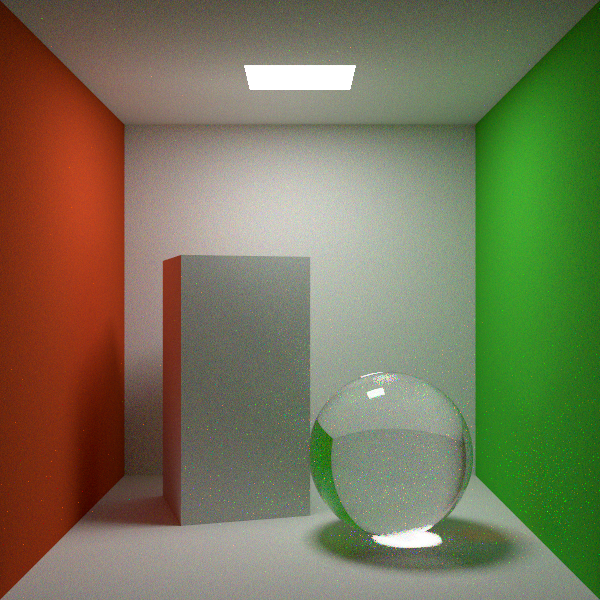
\includegraphics[width=\linewidth]{pt-cornell-box.png}\\[-2pt]
    \small\datei{cornell-box.rttf}
  \end{minipage}\hfill
  \begin{minipage}[b]{0.48\linewidth}\centering
    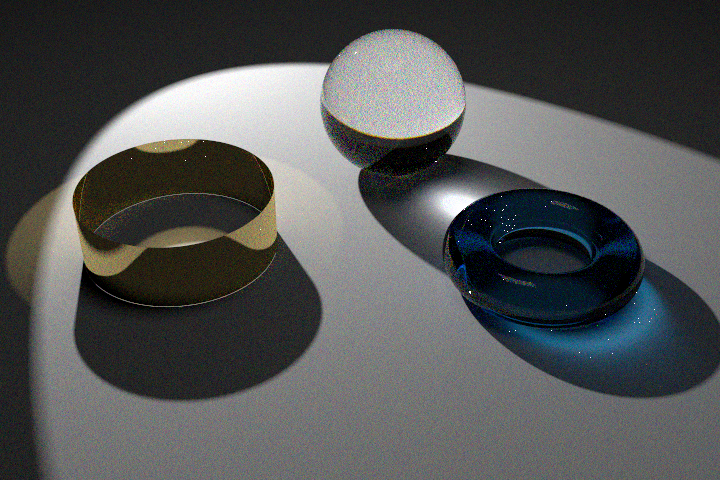
\includegraphics[width=\linewidth]{pt-caustics.png}\\[-2pt]
    \small\datei{caustics.rttf}
  \end{minipage}\\[8pt]
  \begin{minipage}[b]{0.48\linewidth}\centering
    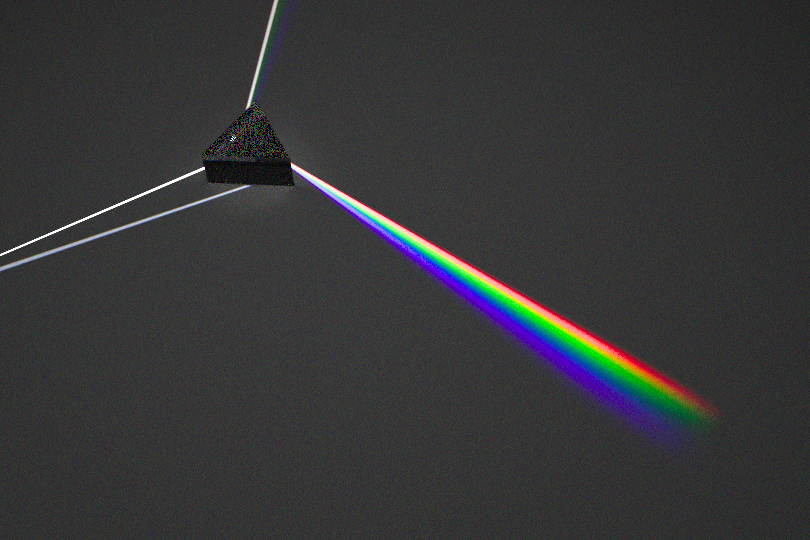
\includegraphics[width=\linewidth]{pt-prism.png}\\[-2pt]
    \small\datei{prism.rttf}
  \end{minipage}\hfill
  \begin{minipage}[b]{0.48\linewidth}\centering
    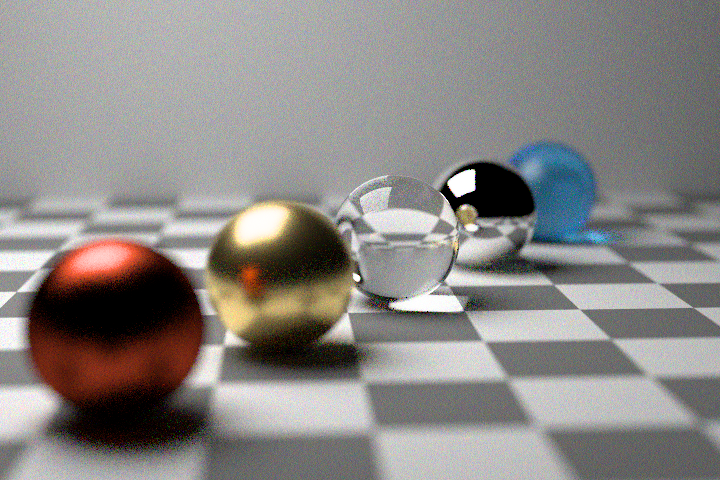
\includegraphics[width=\linewidth]{pt-depth-of-field.png}\\[-2pt]
    \small\datei{depth-of-field.rttf}
  \end{minipage}
  \caption{Farbbilder der vier Beispieldokumente des Path Tracers.}
  \label{fig:pt-beispiele}
\end{figure}

\begin{description}
  \item[\datei{cornell-box.rttf}] Ein Raum von \SI{550}{\milli\metre} mit roter und grüner Wand,
    einer Lampe in der Decke, einem Block und einer Glaskugel: Die Wände färben das Licht, das sie
    weitergeben; die Kugel wirft eine Kaustik. Reflexionsgrade je Wellenlänge, bidirektional.
  \item[\datei{caustics.rttf}] Ein Spot auf einem Tisch, eine Kugel aus stark dispergierendem Glas
    (Abbe-Zahl 28), ein Ring aus blauem Glas (Absorption je Wellenlänge) und ein Band aus poliertem
    Gold: Die Kugel sammelt das Licht in einem hellen Fleck mit farbigen Rändern, das Band erzeugt
    die herzförmige Kurve einer Kaffeetasse. Bidirektional.
  \item[\datei{prism.rttf}] Ein dünnes Band weißen Lichts streift einen Tisch und trifft ein Prisma
    aus Schwerflint ($n = 1{,}785$, Abbe-Zahl 25{,}7) unter dem Winkel minimaler Ablenkung: Die
    Farben verlassen es als Fächer, 31 Wellenlängen von 400 bis \SI{700}{\nano\metre}.
    Bidirektional.
  \item[\datei{depth-of-field.rttf}] Fünf Kugeln auf kariertem Boden unter weichem Licht -- roter
    Lack (glossy), gebürstetes Gold (metal), Glas, ein Spiegel und mattiertes blaues Glas --, durch
    eine Linse von \SI{14}{\milli\metre} Radius gesehen, scharf auf der Glaskugel. Path Tracing.
\end{description}

Die Dokumente verlangen 120 bis 160 Samples je Pixel. Mit dem C++-Kern dauert das auf einem
Laptop mit sechs Kernen etwa eine halbe Minute (Schärfentiefe) bis einige Minuten (Cornell-Box),
mit dem NumPy-Kern weit länger -- verringern Sie dort \gui{Samples} oder die Pixel der Kamera.

\section{Typische Arbeitsabläufe}\label{sec:pt-ablaeufe}

\subsection{Beleuchtungsstärke auf einem Arbeitstisch}

\begin{schritte}
  \item Konstruieren Sie Tisch, Raum (als Flächen oder Körper) und die Leuchtfläche der Leuchte.
  \item Ergänzen Sie die Quellentabelle: Name \code{leuchte}, \gui{Flux} 3000, \gui{in} \code{lm},
    \gui{Wavelengths / nm} z.\,B. \code{450:1, 550:2, 650:1}, \gui{Luminaire file} der Pfad der
    IES-Datei des Herstellers.
  \item Leuchtfläche auswählen, \gui{Source for the selection} = \code{leuchte},
    \gui{Selection: make it a source}.
  \item Wände und Decke: \code{white}; Boden: ein eigenes Material mit Reflexionsgrad 0{,}2.
  \item \gui{Show light paths}: Leuchtet die Leuchte nach unten? Wenn nicht: \gui{Side} auf
    \code{back} stellen.
  \item Tischplatte auswählen, bei \gui{Irradiance on} \gui{Use selection}.
  \item \gui{Results in} = \code{photometric (lm)}, \gui{Method} = \code{light tracing},
    \gui{Irradiance}. Die Tischplatte zeigt die Beleuchtungsstärke in lx, die Tabelle Mittel- und
    Höchstwert.
  \item Ist das Rauschen in der Tabelle zu groß, vervierfachen Sie \gui{Samples}.
\end{schritte}

\subsection{Ein Kamerabild einer Konstruktion}

\begin{schritte}
  \item Materialien zuweisen; eine große Fläche über der Szene als Quelle (\code{lamp}, Halbwinkel
    \SI{90}{\degree}).
  \item \gui{Position} und \gui{Looks at} mit \gui{Pick} setzen, \gui{Show camera} zur Kontrolle.
  \item Für eine erste Vorschau: \gui{Width} 160, \gui{Height} 120, \gui{Samples} 200\,000,
    \gui{Method} \code{path tracing}.
  \item \gui{Camera image}. Ist die Ansicht richtig, Pixel und Samples erhöhen.
  \item Enthält die Szene Glas oder Spiegel mit kleinen Quellen: \code{bidirectional}.
\end{schritte}

\subsection{Eine Kaustik hinter einer Linse}

\begin{schritte}
  \item Linse als geschlossener Körper, Material \code{BK7}.
  \item Kleine Quelle (z.\,B. ein Punkt oder eine kleine Fläche mit kleinem Halbwinkel) vor der
    Linse; mehrere Wellenlängen, wenn Farbfehler sichtbar werden sollen.
  \item Hinter der Linse eine Fläche mit Material \code{white} oder -- wenn sie das Licht nicht
    zurückwerfen soll -- \code{detector}.
  \item \gui{Irradiance on} = diese Fläche, \gui{Method} = \code{light tracing}, \gui{Texels}
    256, \gui{Irradiance}.
  \item Mit \gui{Also per wavelength} sehen Sie die Kaustik jeder Wellenlänge einzeln.
\end{schritte}

\subsection{Verfahren vergleichen}

\begin{schritte}
  \item Dieselbe Szene mit \code{light tracing} und \code{bidirectional} rechnen (gleiche Samples).
  \item In der Tabelle \enquote{Irradiance per face} die Flüsse vergleichen: Sie sollten innerhalb
    von etwa zwei Standardfehlern übereinstimmen.
  \item Weichen sie stärker ab, so findet eines der Verfahren bestimmte Pfade nicht
    (\autoref{sec:pt-verfahren}), oder \gui{Longest path} ist zu kurz.
\end{schritte}

\section{Fehlerbilder und Abhilfe}\label{sec:pt-fehler}

\begin{referenz}{@{}>{\raggedright\arraybackslash}p{0.4\linewidth} >{\raggedright\arraybackslash}X@{}}
\toprule
Meldung oder Beobachtung & Ursache und Abhilfe \\
\midrule\endhead
\texttt{Select surfaces or trimmed surfaces or shells first.} (bzw. mit \texttt{curves or points}) & Nichts Passendes ausgewählt. Objekte auswählen, dann die Aktion wiederholen. \\
\texttt{The material … is not in the table of materials.} & Der Name in \gui{Material for the selection} steht nicht in der Tabelle. \\
\texttt{The source … is not in the table of sources.} & Der Name in \gui{Source for the selection} steht nicht in der Tabelle. \\
\texttt{no object is a source: …} & Kein Objekt verweist auf eine Quelle. Objekt auswählen, \gui{Selection: make it a source}. \\
\textit{Objekt}\texttt{: its material … is not in the table of materials} & Material umbenannt oder gelöscht; neu zuweisen. \\
\texttt{the default material … is not in the table of materials} & \gui{Material of the other objects} nennt kein Material der Tabelle. \\
\texttt{sources need different, non-empty names} & Zwei Quellen heißen gleich oder eine hat keinen Namen. \\
\texttt{source …: a surface already belongs to another source} & Eine Fläche darf nur zu einer Quelle gehören. \\
\texttt{source … is on objects of different kinds …} & Eine Quelle auf Flächen \emph{und} Kurven/Punkten -- in zwei Quellen aufteilen. \\
\texttt{source …: a detector cannot be a source …} & Einer Leuchtfläche ist das Material \code{detector} zugewiesen. \\
\texttt{material …: reflectance + transmittance must lie in 0 … 1} & Werte der Zeile korrigieren. \\
\texttt{camera: position and target are the same point} & \gui{Position} und \gui{Looks at} unterscheiden sich nicht. \\
\texttt{camera: the view direction is parallel to the up direction} & Anderes \gui{Up} wählen. \\
\texttt{the model has no surfaces or bodies to trace} & Nur Kurven/Punkte im Modell oder alles inaktiv. \\
\texttt{luminaire file …: …} & Datei fehlt oder hat ein nicht unterstütztes Format (nur IES Typ C, EULUMDAT). \\
\texttt{The C++ kernel is not installed …} & Paket \code{pathtracer} installieren oder \gui{Kernel} = \code{automatic}. \\
Spiegel oder Glas im Kamerabild schwarz & \code{light tracing} erreicht eine Lochkamera nicht über Spiegel/Glas. \code{bidirectional} oder \code{path tracing} wählen. \\
Kaustik im Kamerabild fehlt, obwohl sie in der Textur zu sehen ist & Sie wird durch Glas oder im Spiegel gesehen: \code{photon mapping}. \\
Punktquelle im Kamerabild unsichtbar & Eine Lochkamera sieht Punktquellen nicht; \gui{Lens radius} $> 0$ und \code{light tracing} oder \code{bidirectional}. \\
Bild zu dunkel, nur einzelne helle Punkte & \gui{White at percentile} senken; mehr Samples. \\
Glaskörper verhält sich falsch & Körper nicht geschlossen; als geschlossenen Körper konstruieren. \\
Rechnung bricht mit Speichermangel ab & \gui{Processes} verringern (NumPy-Kern) oder den C++-Kern verwenden. \\
\bottomrule
\end{referenz}

\section{Grenzen}\label{sec:pt-grenzen}

\begin{itemize}
  \item Keine kontinuierlichen Spektren und Farben: Gerechnet wird mit einzelnen Linien.
  \item Keine gemessenen Materialien (BRDF-Daten).
  \item Quellen und Kameras dürfen nicht in Glas liegen.
  \item Ergebnisse werden nicht mit dem Dokument gespeichert; dafür gibt es \gui{Also write to
    file}.
  \item Kurven und Punkte als Quellen werfen keinen Schatten und sind für die Kamera unsichtbar.
\end{itemize}
